% Be sure to set \appendix or \appendices in structural/body.tex
%\chapter{Some theoretical background}
%\label{app.theory}
%Unlike Classical particles, elementary particles obey the laws of quantum mechanics and special relativity. Combining both theories gives {\it quantum field theory}, which is the backbone of the Standard Model. In this appendix, we present a simplified overview of important concepts in quantum mechanics and special relativity. (This is appendix is by no means a comprehensive review, but may hopefully provide some context for background knowledge mentioned in the body of this thesis.) For undergraduates interested in learning more about the theories, below are a few textbook recommendations:
%\begin{itemize}
%    \item Quantum mechanics:
%    \begin{itemize}
%        \item {\it Introduction to Quantum Mechanics} by Griffiths \& Schroeter \cite{Griffiths_Schroeter}
%    \end{itemize}
%    \item Special relativity, quantum field theory, and particle physics: 
%    \begin{itemize}
%        \item {\it Introduction to Elementary Particles} by Griffiths \cite{Griffiths}
%        \item {\it A Standard Model Workbook} by Moore \cite{Moore}=
%        \item {\it Quarks \& Leptons: An Introductory Course in Modern Particle Physics} by Halzen \& Martin \cite{Halzen_Martin}
%    \end{itemize}
%\end{itemize}

%-------------------------
%\section{Quantum mechanics}
%\label{sec.quantum}

%At very small distance scales, systems are governed by quantum physics, exhibiting both particle-like and wave-like properties. In quantum mechanics, the state of a system is given by a {\it wavefunction} $\ket{\psi}$, which is a vector in a complex-valued vector space, called Hilbert space. $\ket{\psi}$ obeys all the properties of vectors. In particular, it can be written as a linear combination of vectors in any basis of our choice.

%Additionally, $\ket{\psi}$ evolves in time according the {\it Schrodinger equation}, which is a wave equation, and thus also obeys all the properties of waves. For example, wavefunctions propagate and interfere with each other. In the common position-basis, the {\it amplitude} of the wavefunction is given by $\psi(\mathbf{x},t)$, and the Schrodinger equation looks like
%\begin{equation}
%    i\frac{\partial}{\partial t}\psi(\mathbf{x},t) = -\frac{1}{2m}\nabla^2\psi(\mathbf{x},t) + V(\mathbf{x})\psi(\mathbf{x},t) \ ,
%\end{equation}
%where the spatial derivative term represents the kinetic energy, and the $V(\mathbf{x})$ term represents the potential energy.
% For a free particle, where $V(\mathbf{x})=0$, the wavefunction is a {\it plane wave},
% \begin{equation}
%     \psi(\mathbf{x},t)=Ae^{i(\mathbf{p}\cdot\mathbf{x}-Et)} \ ,
% \end{equation}
% where $\mathbf{p}$ is the momentum of the particle, $E$ is the total energy of the particle, and $A$ is a normalization constant chosen such that
% \begin{equation}
%     |\psi(\mathbf{x},t)|^2=1 \ .
% \end{equation}
% Thus, we interpret $\psi(\mathbf{x},t)$ as a {\it probability amplitude}.

%Another condition that wavefunctions must satisfy is {\it normality}, given by
%\begin{equation}
%    |\braket{\psi|\psi}|^2 \equiv 1 \ , 
%    \label{eqn.norm}
%\end{equation}
%or, in terms of the position basis amplitude,
%\begin{equation}
%    \int_{-\infty}^\infty d^3\mathbf{x} \ |\psi(\mathbf{x},t)|^2 \equiv \int_{-\infty}^\infty d^3\mathbf{x} \ \psi^*(\mathbf{x},t)\psi(\mathbf{x},t) \equiv 1 \ .
%    \label{eqn.norm2}
%\end{equation}
%Eq. \eqref{eqn.norm} and \ref{eqn.norm2} define the inner product of the wavefunction with itself, which is equal to its magnitude squared. (This is analogous to taking the inner product, or dot product, of the vector $\mathbf{x}=(x,y,z)$, which gives the length of the vector squared: $|\mathbf{x}|^2\equiv\mathbf{x}\cdot\mathbf{x}=x^2+y^2+z^2$. In Eq. \eqref{eqn.norm2}, $\psi(\mathbf{x},t)$ is a complex-valued function, so the inner product also includes an integral and complex conjugation.)

%Since the integral in Eq. \eqref{eqn.norm2} is equal to 1, we interpret $|\psi(\mathbf{x},t)|^2$ as a probability density, and $\psi(\mathbf{x},t)$ as a {\it probability amplitude}. More generally, the inner product of any two states $\ket{\psi_1}$ and $\ket{\psi_2}$, denoted $\braket{\psi_1|\psi_2}$ or $\braket{\psi_2|\psi_1}$, represents a probability. For example, in order to determine the probability of a system transitioning from some initial state $\ket{\psi_i}$ to some final state $\ket{\psi_f}$, we take the squared inner product $|\braket{\psi_f|\psi_i}|^2={\rm Prob}_{i\rightarrow f}$. In fact, in high energy experiments, many measurements boil down to determining the probability that some initial set of particles transitions into some final set of particles after they collide.

% {\color{brown} Due to the probabilistic nature of quantum mechanics, particles and systems do not have definite properties, such as position, momentum, energy, etc., until we ``observe" them, or measure them. When we perform a measurement, our interaction with the system {\it collapses} the wavefunction into a definite state..........

 % Heisenberg uncertainty principle? Observables?}
% \begin{itemize}
%     \item measurement and wavefunction collapse (system becomes particle-like)
% \end{itemize}

%---------------------------------------------------------
\chapter{Some concepts in special relativity}
\label{sec.relativity}
Unlike Classical particles, elementary particles obey the laws of quantum mechanics and special relativity. Combining both theories gives {\it quantum field theory}, which is the backbone of the Standard Model. In this appendix, we present a simplified overview of important concepts in special relativity, which may serve to provide context for some of the background knowledge mentioned in the body of this thesis.
%For undergraduates interested in learning more about the theories, below are a few textbook recommendations:
%\begin{itemize}
%    \item Special relativity, quantum field theory, and particle physics: 
%    \begin{itemize}
%        \item {\it Introduction to Elementary Particles} by Griffiths \cite{Griffiths}
%        \item {\it A Standard Model Workbook} by Moore \cite{Moore}=
%        \item {\it Quarks \& Leptons: An Introductory Course in Modern Particle Physics} by Halzen \& Martin \cite{Halzen_Martin}
%    \end{itemize}
%\end{itemize}

%-------------------------
\section{Four-vectors and Lorentz transformations}
When objects travel near the speed of light, as particles do in high energy experiments, they obey relativistic physics. In special relativity, space and time are treated on equal footing, as coordinates in {\it spacetime} (also known as Minkowski space). Position $\mathbf{x}$ and time $t$ are then combined into a new object, called a {\it four-vector},
\begin{equation}
    \tilde x \equiv \begin{pmatrix}
        t \\
        \mathbf{x}
    \end{pmatrix}\
    =\begin{pmatrix}
        t \\
        x \\
        y \\
        z
    \end{pmatrix}\ . \label{eqn.xmu}
\end{equation}
Like any other type of vector, four-vectors can be added, scaled, and transformed via linear transformations, or matrices. (Commonly, bold-faced symbols like $\mathbf{x}$ are used to denote ``regular" three-dimensional vectors while four-vectors are denoted with non-bold symbols like $x$. Here, we instead use $\tilde{x}$ to denote the position four-vector in order to avoid confusion with the coordinate $x$.) In standard notation, the components of a four-vector are denoted $\tilde x^\mu$, where the index $\mu=0,1,2,3$ acts as a label. For example, $\tilde{x}^0=t$ for $\mu=0$, $\tilde{x}^1=x$ for $\mu=1$, etc.

If we want to change from one reference frame to another, we must apply a rotation of the spacetime coordinates, known as a {\it Lorentz transformation}. In other words, we need to rotate the four-vector $\tilde{x}$. To implement transformations on a four-vector, we need $4\times 4$ matrices of the form
\begin{equation}
    M = \begin{pmatrix}
        M^0_0 & M^0_1 & M^0_2 & M^0_3 \\
        M^1_0 & M^1_1 & M^1_2 & M^1_3 \\
        M^2_0 & M^2_1 & M^2_2 & M^2_3 \\
        M^3_0 & M^3_1 & M^3_2 & M^3_3 \\
    \end{pmatrix} \ ,
\end{equation}
where $M^\mu_\nu$ is the element in row $\mu$ column $\nu$, with $0$ being the time index and $1,2,3$ being the $x,y,z$ indices. Regular spatial rotations, such as
\begin{equation}
    \Lambda_R = \begin{pmatrix}
        1 & 0 & 0 & 0 \\
        0 & \cos{\theta} & -\sin{\theta} & 0 \\
        0 & \sin{\theta} & \cos{\theta} & 0 \\
        0 & 0 & 0 & 1
    \end{pmatrix} \ ,
\end{equation}
which rotates a four-vector about the $z$-axis by some angle $\theta$, are a form of Lorentz transformation. (Remember the $0$-th row and column correspond to time.) 

Additionally, there is another type of Lorentz transformation, called a {\it boost}, which allows us to transform between two reference frames that are moving relative to each other. For example, consider a particle traveling at velocity $\beta$ in the $+x$ direction relative to a stationary observer. From the stationary observer's frame, we can boost into the moving particle's frame by multiplying all the coordinates by the Lorentz transformation matrix
\begin{align}
    \Lambda_B = \begin{pmatrix}
        \gamma & -\gamma\beta & 0 & 0 \\
        -\gamma\beta & \gamma & 0 & 0 \\
        0 & 0 & 1 & 0 \\
        0 & 0 & 0 & 1 
    \end{pmatrix} \ , \label{eqn.boost}
\end{align}
where $\gamma = 1/\sqrt{1-\beta^2}$. (Note that in natural units, the speed of light is $c=1$. Particles cannot travel faster than the speed of light, so $\beta \leq 1$, which means $\gamma \ge 1$.) 

%-------------------------
\section{The relativity of time and distance}
Suppose we, as the stationary observer, measure the time and distance traveled by a particle (which is moving with velocity $\beta$) to be $\Delta\tilde x=(\Delta t, \Delta x, \Delta y, \Delta z)$. If we boost to the particle's frame, we will see that the particle measures its own travel time and distance to be $\Delta\tilde x'=(\Delta t', \Delta x', \Delta y', \Delta z')$, where
\begin{equation}
    \begin{pmatrix}
        \Delta t' \\
        \Delta x' \\
        \Delta y' \\
        \Delta z'
    \end{pmatrix}
    = \begin{pmatrix}
        \gamma & -\gamma\beta & 0 & 0 \\
        -\gamma\beta & \gamma & 0 & 0 \\
        0 & 0 & 1 & 0 \\
        0 & 0 & 0 & 1 
    \end{pmatrix}
    \begin{pmatrix}
        \Delta t \\
        \Delta x \\
        \Delta y \\
        \Delta z
    \end{pmatrix} \\
    = \begin{pmatrix}
        \gamma(\Delta t-\beta\Delta x) \\
        \gamma(-\beta \Delta t + \Delta x) \\
        \Delta y \\
        \Delta z
    \end{pmatrix} \ .
    \label{eqn.lorentz}
\end{equation}
In general, Eq. \eqref{eqn.lorentz} shows that measurements made by two observers do not agree if they are traveling with relative motion between them. Thus, distances and time intervals are no longer absolute, but are relative.

Two important consequences of relativity are {\it time dilation} and {\it length contraction}. Roughly speaking, time dilation describes the phenomenon in which a moving observer will experience time passing more slowly relative to a stationary observer. Length contraction describes the phenomenon in which the length of a moving object will be shortened along its direction of motion. In high energy collisions, this means that unstable particles traveling near the speed of light live longer than their average lifetimes (as measured for the particles at rest), and they become ``pancaked" along their direction of travel. The larger the $\gamma$ (or velocity $\beta$), the stronger the effects.

%-------------------------
\section{Lorentz-invariance}
Although distances and time are now relative, there is still a way to define absolute lengths. In normal three-dimensional space, we measure lengths by taking the dot product of the position vector $\mathbf{x}$ with itself, $|\mathbf{x}|^2 = \mathbf{x}\cdot\mathbf{x} = x^2+y^2+z^2$. In spacetime, distances are given by the inner product of a four-vector with itself, which is defined
\begin{equation}
\begin{aligned}
    \tilde{x}^2 &= \tilde{x}\cdot\tilde{x} \equiv t^2 - \mathbf{x}^2 \\
    &= t^2-x^2-y^2-z^2 \ . 
\end{aligned}
\end{equation}
Note that there is a relative sign difference between the time component and spatial components. The reason we define the inner product this way is because this quantity is actually {\it Lorentz-invariant}, meaning that its value is the same in every reference frame. 

More generally, the inner product of any four-vector object with itself is Lorentz-invariant. One important example is the momentum four-vector,
\begin{equation}
    p \equiv \begin{pmatrix}
        E \\
        \mathbf{p}
    \end{pmatrix}
    = \begin{pmatrix}
        E \\
        p_x \\
        p_y \\
        p_z
    \end{pmatrix}
    = \begin{pmatrix}
        \gamma m \\
        \gamma m v_x \\
        \gamma m v_y \\
        \gamma m v_z
    \end{pmatrix}\ , \label{eqn.four_momentum}
\end{equation}
where $E$ is energy, and $\mathbf{p}$ is the three-dimensional momentum vector, $m$ is mass, and $\mathbf{v}=(v_x,v_y,v_z)$ is the three-dimensional velocity vector. The $\gamma$ factor accounts for the relativistic motion. For particles traveling with small momenta, $\gamma\approx 1$, and $p\approx(m, mv_x,mv_y,mv_z)$.
\begin{equation}
\begin{aligned}
    p^2 = p \cdot p &= E^2-|\mathbf{p|^2} \\
    &=  \gamma^2m^2(1-|\mathbf{v}|^2) = \frac{1}{1-\beta^2}m^2(1-\beta^2) \\
    &= m^2,
    \label{eqn.mass}
\end{aligned}
\end{equation}
Putting back the factors of $c$, Eq. \eqref{eqn.mass} reads $E^2-(|\mathbf{p}|c)^2 = (mc^2)^2$. In the rest frame of a particle (in which $\mathbf{p}=0$), this reduces to Einstein's famous equation $E=mc^2$. 

Lorentz-invariance is essential, as it ensures that the laws of physics are the same in every reference frame. Thus, when describing high-energy particle traveling near the speed of light, we must take care that all our equations are built from Lorentz-invariant quantities.

%-------------------------
\section{Rapidity}
In analogy to spatial rotations, we can also write a Lorentz boost as a hyperbolic rotation between space and time. For example, a boost along the $x$-direction is given by
\begin{align}
    \Lambda_B = \begin{pmatrix}
        \cosh{y} & -\sinh{y} & 0 & 0 \\
        -\sinh{y} & \cosh{y} & 0 & 0 \\
        0 & 0 & 1 & 0 \\
        0 & 0 & 0 & 1
    \end{pmatrix} \ , \label{eqn.boost2}
\end{align}
where
\begin{equation}
    y\equiv \tanh^{-1}(\beta) \label{eqn.y}
\end{equation}
is called the {\it rapidity}. (Eq. \eqref{eqn.boost2} represents the exact same transformation as Eq. \eqref{eqn.boost}.) Just like $\theta$ determines the amount by which a spatial rotation is performed, the rapidity $y$ determines how much a four-vector is boosted. The greater the relative velocity $\beta$ between two reference frames, the larger the $y$, and the greater the boost must be to go from one to the other. 

The more common expression for rapidity in particle physics is
\begin{equation}
    y = \frac{1}{2}\ln \left[ \frac{E+p_z}{E-p_z} \right] \ , \label{eqn.y2}
\end{equation}
written in terms of the energy $E$ and momentum $p_z$ of a particle. (We can always define the $z$-direction to be the particle's direction of motion relative to us.) We can see that Eq. \eqref{eqn.y} and \eqref{eqn.y2} are equivalent:
\begin{equation}
\begin{aligned}
    y &= \tanh^{-1}(\beta) \\
    &= \frac{1}{2}\ln \left[ \frac{1+\beta}{1-\beta} \right] \\
    &= \frac{1}{2}\ln \left[ \frac{\gamma m(1+\beta)}{\gamma m(1-\beta)} \right] \\
    &=\frac{1}{2}\ln \left[ \frac{E+p_z}{E-p_z} \right] \ ,
\end{aligned}
\end{equation}
where in the second line we have used the definition $\tanh^{-1}x = \ln [(1+x)/(1-x)]$, and in the last line we have used the definition of $E$ and $\mathbf{p}$ in Eq. \eqref{eqn.four_momentum} for a particle traveling in the $z$-direction.

One useful property of $y$ is that it is Lorentz-invariant, since it is specifically defined for two particular reference frames, whose relative velocity is always $\beta$. (Absolute velocities are not Lorentz-invariant, but relative velocities are.) Additionally, since $y$ is equal to the natural log of some quantity, as written in Eq. \eqref{eqn.y2}, rapidities obey simple addition and subtraction, and we do not need to deal with complicated Lorentz transformations like we would in order to add regular velocities.  Thus, we can think of rapidity as a ``relativistic version" of velocity that is easier to work with in particle physics.

%----------------------------------------------------------
% \chapter{Point-like scattering: the elastic $e\mu$ cross section}
% \label{app.emu}

% This interaction is mediated by a virtual photon, whose four-momentum $q\equiv(\nu, \mathbf{q})=k-k'$ is equal to the amount of four-momentum transferred between the electron and proton. A quick calculation reveals that
% \begin{equation}
%     q^2 = (k-k')^2 = 2k\cdot k' = 2EE'(1-\cos{\theta}) \ ,
% \end{equation}
% which is in general nonzero. Thus, $q^2\neq m_\gamma^2$, seemingly breaking the laws of relativity. Vaguely speaking, the Heisenberg uncertainty principle $\Delta E \Delta t \geq 1 / 2$ provides some leeway, allowing such particles to fluctuate into existence for an extremely brief, unobservable, amount of time. These particles are termed {\it virtual}, or {\it off-shell}.

%----------------------------------------------------------
\chapter{Data samples}
\label{app.samples}

Here we reference the PYTHIA-8 simulation samples used to complete this thesis, which are provided by the ePIC Collaboration \cite{ePIC}. We obtain signal candidates from ``D0" samples, which refer to $D^0$-enriched data in which every event in the sample contains at least one $D^0$ particle. We obtain background candidates from ``DIS" samples, which refer to minimum-bias data without $D^0$-enrichment.

For the examination of topological distributions in Ch. \ref{ch:d0_top}, we utilize the December 2024 campaign $ep$ simulations.
\begin{enumerate}
    \item D0 samples with $Q^2>1~{\rm GeV^2}$: \\
    /volatile/eic/EPIC/RECO/24.12.0/epic\_craterlake/SIDIS/D0\_ABCONV\\/pythia8.306-1.1/10x100/q2\_1/hiDiv/
    
    \item D0 samples with $Q^2>100~{\rm GeV^2}$: \\
    volatile/eic/EPIC/RECO/24.12.0/epic\_craterlake/SIDIS/D0\_ABCONV\\/pythia8.306-1.1/10x100/q2\_1/hiDiv/
    
\end{enumerate}

For machine learning analyses in Ch. \ref{ch.results}, we utilize the October 2025 campaign $ep$ simulations with $Q^2>1~{\rm GeV^2}$.
\begin{enumerate}
    \item Samples without machine-background effects
    \begin{enumerate}
        \item D0 samples: \\
        /volatile/eic/EPIC/RECO/25.10.3/epic\_craterlake/SIDIS/D0\_ABCONV\\/pythia8.306-1.1/10x100/q2\_1/hiDiv/
        
        \item DIS samples: \\
        /volatile/eic/EPIC/RECO/25.10.0/epic\_craterlake/DIS/NC/10x100\\/minQ2=1/

    \end{enumerate}
    \item Samples \textbf{with} machine-background effects
    \begin{enumerate}
        \item D0 samples: \\
        /volatile/eic/EPIC/RECO/25.10.4/epic\_craterlake\\/Bkg\_Exactly1SignalPer2usFrame/SIDIS/D0\_ABCONV\\/pythia8.306-1.1/10x100/q2\_1/hiDiv/
        
        \item DIS samples: \\
        /volatile/eic/EPIC/RECO/25.10.4/epic\_craterlake\\/Bkg\_1SignalPer2usFrame/DIS/NC/10x100/minQ2=1/

    \end{enumerate}
\end{enumerate}

The codes to obtain signal and background candidates are found in the directory \texttt{ML\_by\_slices/analysis\_jobs/} of the GitHub repository for this thesis \cite{github}, which is based on the analysis frameworks provided by Shyam Kumar \cite{Shyam_analysis} and Rongrong Ma \cite{Rongrong_jobs}.

%----------------------------------------------------------
\chapter{Data preparation for BDT and $D^0$ invariant mass plots}
\label{app.data_prep}

In this appendix, we describe the procedures to prepare the data for training BDT and plotting invariant mass distributions, after obtaining the signal and background candidates. The codes to implement the procedures are found in the Jupyter notebook \texttt{ML\_by\_slices/ML\_example\_results/ML\_by\_slices.ipynb} in our GitHub repository \cite{github} and is adapted from the machine learning framework provided by Shyam Kumar \cite{Shyam_ml}.

Here, we list the general steps and expand upon them in the following sections.
\begin{enumerate}
    \item Apply broad preselections, and select $y$ and $p_T$ ranges
    \item Fit $D^0$ invariant mass distributions of signal and background candidates
    \item Plot $D^0$ invariant mass distribution before BDT
    \begin{enumerate}
        \item Calculate the numbers of signal and background candidates expected for the desired number of events
        \item Randomly sample signal and background candidates from the fits
    \end{enumerate}
    \item Select signal and background datasets for BDT training
    \item Plot $D^0$ invariant mass distribution after BDT
    \begin{enumerate}
        \item Calculate the expected numbers of signal and background candidates selected by BDT
        \item Randomly sample signal and background candidates from the fits
    \end{enumerate}
\end{enumerate}


%------------------------
\section{Preselection and kinematic cuts}
\label{app.presel}
To reduce the size of the data we need to deal with, we first apply the following preselections on both signal and background candidates:
\begin{itemize}
    \item $1.6 < m_{D^0} < 2.5 ~{\rm GeV/c^2}$
    \item $0.02 < {\rm DCA_\pi}_{(xy)} < 10 ~{\rm mm}$
    \item $0.02 < {\rm DCA_K}_{(xy)} < 10 ~{\rm mm}$
    \item ${\rm Decay~Length} < 100 ~ {\rm mm}$
\end{itemize}
These broad cuts remove (mostly background) candidates far away from the expected $D^0$ invariant mass peak (around $1.86~{\rm GeV/c^2}$).

We then apply cuts on the $y$ and $p_T$ of the candidates to select the kinematic slice of interest.

%------------------------
\section{Training and testing data selections for BDT}
\label{app.presel}
We train the models on the ``raw" data obtained after preselection and kinematic cuts (not on the resampled data.) For training, we want the numbers of signal and background candidates to be the same. Thus, we resize the signal and background datasets (using randomized selection) to equal the minimum number of the two.

We also make additional invariant mass cuts on the signal and background candidates such that the signal candidates sit in or near the expected $D^0$ peak region and the background candidates sit in the sideband regions:
\begin{itemize}
    \item Signal cut: $1.7 < m_{D^0}<2.1$
    \item Background cut: $1.6 < m_{D^0}<1.7$ or $2.1 < m_{D^0}<2.5$
\end{itemize}

%------------------------
\section{Fits and resampling}
\label{app.resamp}

To produce the $D^0$ invariant mass plots, we scale up the number of signal and background candidates so that they correspond to the statistics expected in real EIC experiments. We do this by fitting the $D^0$ invariant mass distributions of the signal and background candidates, then randomly sampling the required numbers of candidates from those fitted distributions. Fig. \ref{f.resamp} illustrates examples of the data along with the fits and resampled distributions.

%
\begin{figure}[h!]
    \centering
    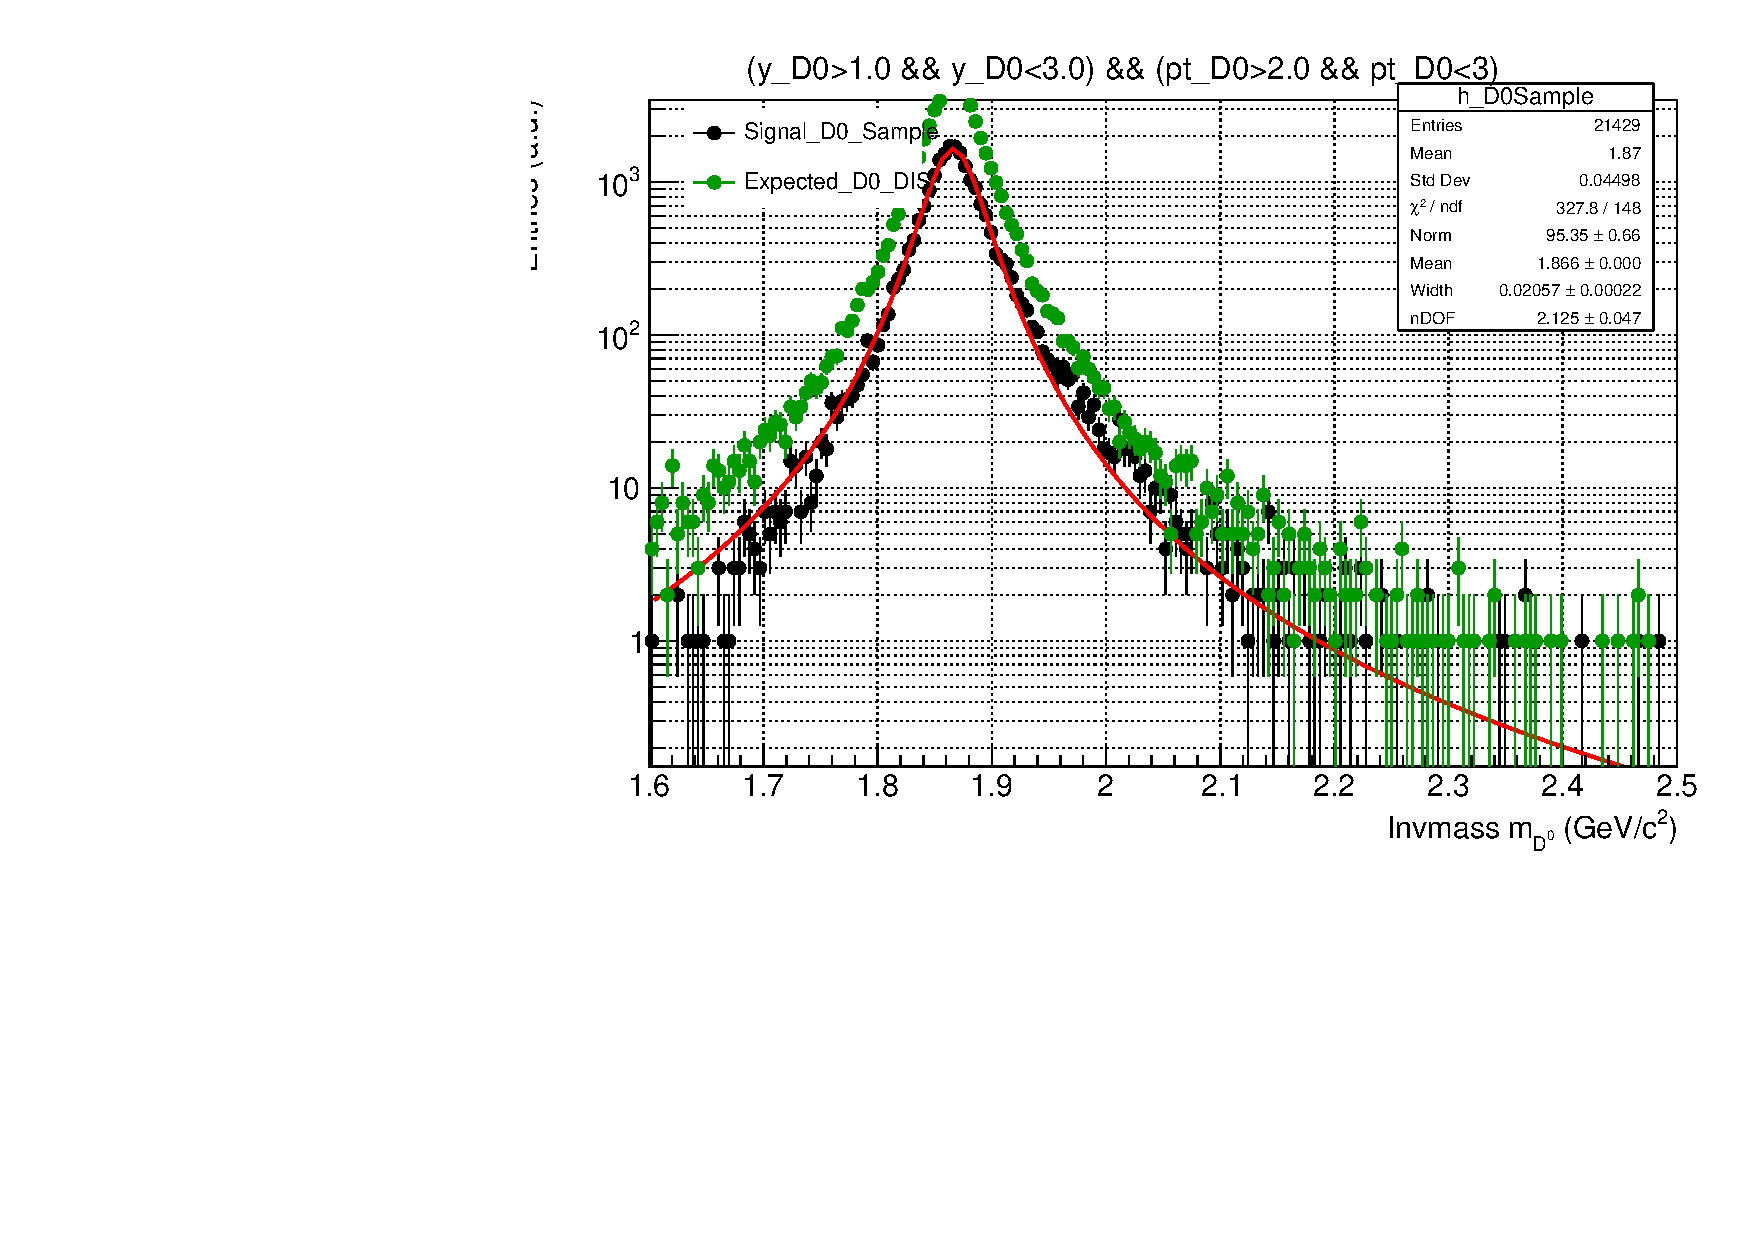
\includegraphics[width=0.6\linewidth]{gallery/appendix/resampled_signal_y_1.0_3.0_pt_2.0_3.0_before_ml.pdf}
    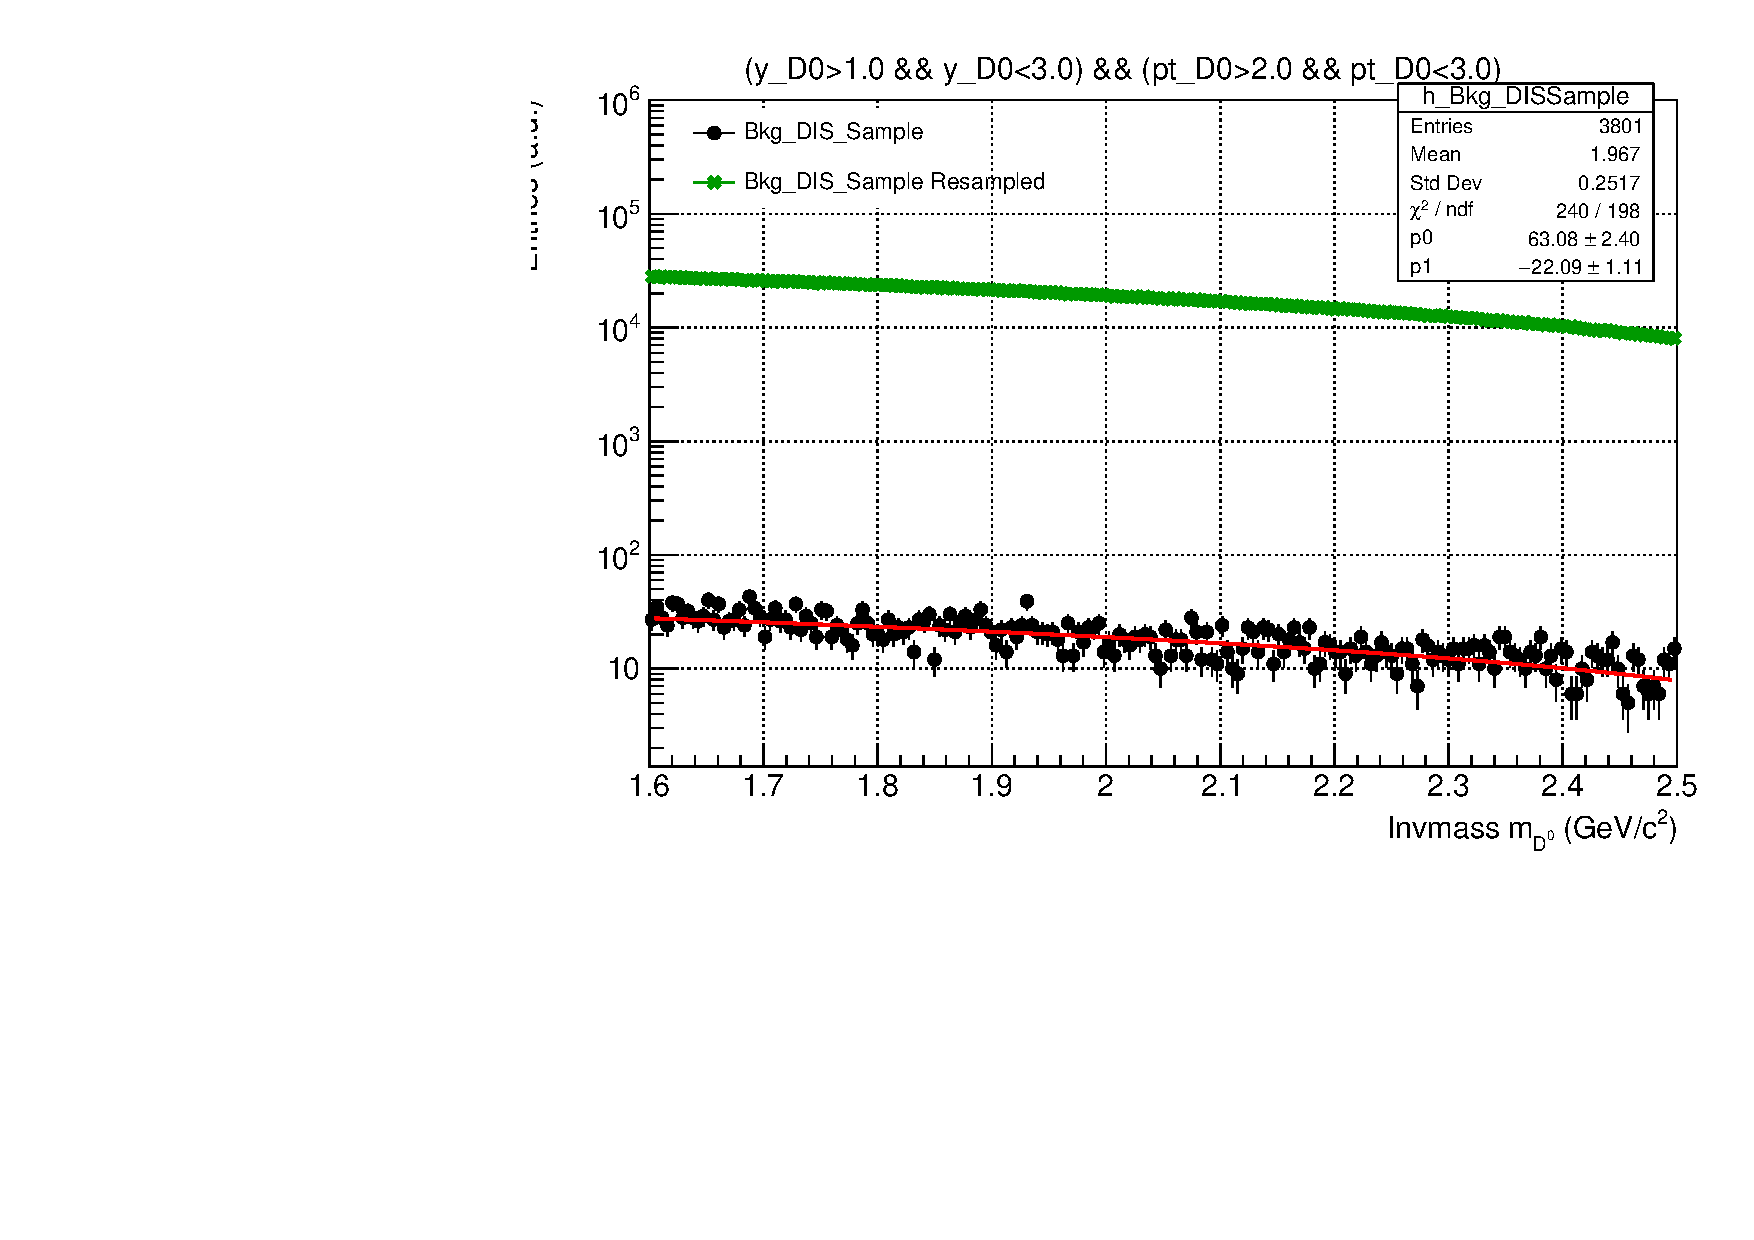
\includegraphics[width=0.6\linewidth]{gallery/appendix/resampled_bkg_y_1.0_3.0_pt_2.0_3.0_before_ml.pdf}
    \caption{Example fits to $D^0$ invariant mass distributions of signal (top) and background (bottom) candidates. Black markers indicate the original data, red curves indicate the fitted functions, and green markers indicate the resampled data. Signal distributions are fit using Student's $t$-distribution $f(x)=N\frac{\Gamma((\nu+1)/2)}{\sqrt{\nu\pi}\sigma\Gamma(\nu/2)}\left(1+\frac{(x-\mu)^2}{\sigma^2}\right)^{-(\nu+1)/2}$ with 4 free parameters: norm $N$, mean $\mu$, width $\sigma$, and nDOF $\nu$. Background distributions are fit using a second-degree polynomial $f(x)=p_0+p_1x+p_2x^2$ with 3 free parameters: $p_0$, $p_1$, and $p_2$.}
    \label{f.resamp}
\end{figure}
%
We fit the original $D^0$ invariant mass distribution (black) of the signal candidates with Student's $t$-distribution,
\begin{equation}
    f(x)={\color{purple} N}\frac{\Gamma(\frac{{\color{purple}\nu}+1}{2})}{\sqrt{{\color{purple}\nu}\pi} \ {\color{purple}\sigma} \ \Gamma(\frac{{\color{purple}\nu}}{2})}\left(1+\frac{(x-{\color{purple}\mu})^2}{{\color{purple}\sigma}^2}\right)^{-({\color{purple}\nu}+1)/2} \ ,
\end{equation}
where the norm $N$, mean $\mu$, width $\sigma$, and degrees of freedom (nDOF) $\nu$ are free parameters fitted to the data by a $\chi^2$ minimization procedure. This is a generalization of a Gaussian distribution with mean $\mu$ and standard deviation $\sigma$. We fit the distribution of background candidates with a second-degree polynomial,
\begin{equation}
    f(x)={\color{purple}p_0}+{\color{purple}p_1}x+{\color{purple}p_2}x^2 \ ,
\end{equation}
with free parameters $p_0$, $p_1$, and $p_2$. The best fit curves are shown in red in Fig. \ref{f.resamp}.

In our analyses, we work with the expected luminosity of $10 ~{\rm fb^{-1}}$, which corresponds to $4.72162\times10^9$ total events in each set of simulation samples. The number of expected background candidates is thus
\begin{equation}
    \hat{N}_{\rm bkg} = \frac{N_{\rm bkg}}{E_{\rm bkg}} \ \hat{E} \ , \label{eqn.Nbkg}
\end{equation}
where $\hat{N}_{\rm bkg}$ is the expected number of background candidates, $N_{\rm bkg}$ is the original number of candidates obtained from the DIS simulation samples, $E_{\rm bkg}$ is the number of events contained in those DIS samples, and $\hat{E} = 4.72162\times10^9$ is the expected total number of events.

The number of expected signal candidates is
\begin{equation}
    \hat{N}_{\rm sig} = \frac{N_{\rm sig}}{E_{\rm sig} S} \ \hat{E} \ , \label{eqn.Nsig}
\end{equation}
where an additional factor $S=1821.83$ is included to scale the number of events in the D0 samples to match that in the DIS samples.

To plot the $D^0$ invariant mass distribution before BDT, we randomly sample $\hat{N}_{\rm bkg}$ candidates from the fitted polynomial distribution and $\hat{N}_{\rm sig}$ candidates from the fitted Student's $t$-distribution, and plot all the candidates together. The resampled distributions are shown in green in Fig. \ref{f.resamp} and combine to form the black distribution for the data before BDT in Fig. \ref{f.inv_mass_ex}. We then calculate the S/B and Significance, 
\begin{align}
    {\rm S/B} &= \frac{\hat{N}_{\rm sig}^{D^0}}{\hat{N}_{\rm bkg}^{D^0}} \\
    {\rm Signif} &= \frac{\hat{N}_{\rm sig}^{D^0}}{\sqrt{\hat{N}_{\rm sig}^{D^0}+\hat{N}_{\rm bkg}^{D^0}}} \ ,
\end{align}
where $\hat{N}_{\rm sig}^{D^0}$ and $\hat{N}_{\rm bkg}^{D^0}$ are obtained by counting the number of resampled candidates within $2\sigma$ on each side of $\mu$ (with $\sigma$ and $\mu$ given by the fitted signal distribution).

%
\begin{figure}[h!]
    \centering
    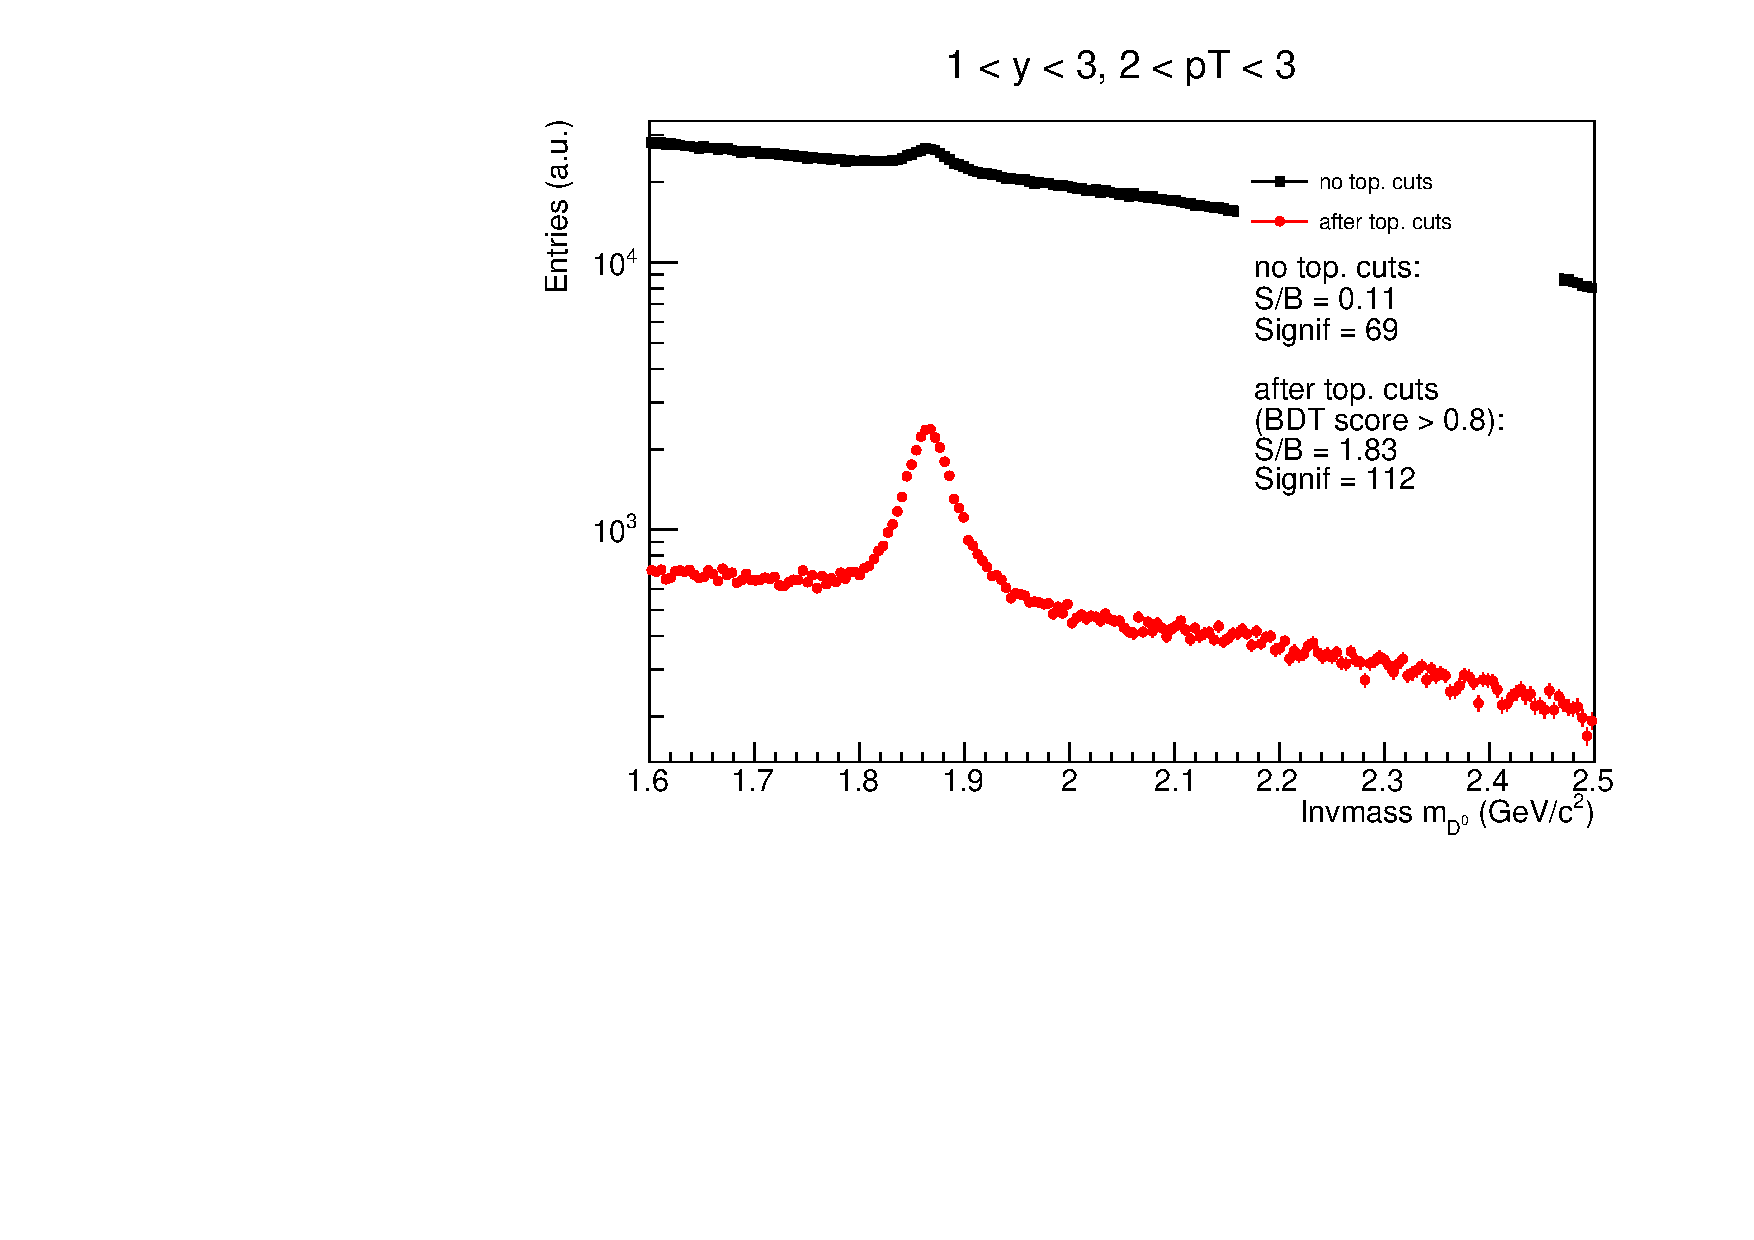
\includegraphics[width=0.7\linewidth]{gallery/appendix/inv_mass_before_and_after_ML_y_1.0_3.0_pt_2.0_3.0_bdt_0.8.pdf}
    \caption{Example $D^0$ invariant mass distributions of resampled candidates before BDT (black) and after BDT (red).}
    \label{f.inv_mass_ex}
\end{figure}
%

After performing the machine learning, we choose a BDT threshold $\hat{y}^*$ and obtain the corresponding efficiencies, $\epsilon_{\rm sig}(\hat{y}^*)$ and $\epsilon_{\rm bkg}(\hat{y}^*)$, which represent the fractions of signal and background candidates selected by the BDT. (The efficiencies are calculated using the raw data, but we generalize the results to the resampled data.) The numbers of resampled candidates after BDT are
\begin{align}
    \hat{N}^{BDT}_{\rm bkg} &= \hat{N}_{\rm bkg} \ \epsilon_{\rm bkg}(\hat{y}^*) \\
    \hat{N}^{BDT}_{\rm sig} &= \hat{N}_{\rm sig} \ \epsilon_{\rm sig}(\hat{y}^*)  \ ,
\end{align}
where $\hat{N}_{\rm bkg}$ and $\hat{N}_{\rm sig}$ are the numbers from Eq. \eqref{eqn.Nbkg} and \eqref{eqn.Nsig}.

To produce the red distribution for the data after BDT in Fig. \ref{f.inv_mass_ex}, we randomly sample $\hat{N}^{BDT}_{\rm sig}$ and $\hat{N}^{BDT}_{\rm bkg}$ candidates from the fitted signal and background distributions (the same ones from which we sampled the data before BDT). Finally, we calculate the S/B and Significance in the same manner as for the data before BDT.
